\documentclass{beamer}
\usetheme{Madrid}
\usecolortheme{default}
\usepackage{listings}
\usepackage{xcolor}
\usepackage{graphicx}
\usepackage{tikz}
\usetikzlibrary{shapes,arrows,positioning,fit,backgrounds}

% Define Jupyter-like syntax highlighting
\definecolor{jupyterblue}{RGB}{0,112,192}
\definecolor{jupytergreen}{RGB}{0,128,0}
\definecolor{jupyterorange}{RGB}{170,85,0}
\definecolor{jupyterpurple}{RGB}{128,0,128}
\definecolor{jupyterbackground}{RGB}{248,248,248}
\definecolor{jupyterborder}{RGB}{204,204,204}

\lstdefinestyle{jupyter}{
    backgroundcolor=\color{jupyterbackground},   
    commentstyle=\color{jupyterorange},
    keywordstyle=\color{jupyterblue},
    stringstyle=\color{jupytergreen},
    basicstyle=\ttfamily\footnotesize,
    breakatwhitespace=false,         
    breaklines=true,                 
    captionpos=b,                    
    keepspaces=true,                 
    numbers=none,                    
    showspaces=false,                
    showstringspaces=false,
    showtabs=false,                  
    tabsize=4,
    frame=single,
    framesep=5pt,
    frameround=tttt, % square corners
    framexleftmargin=5pt,
    framexrightmargin=5pt,
    framextopmargin=5pt,
    framexbottommargin=5pt,
    rulecolor=\color{jupyterborder}
}

\lstset{style=jupyter, language=Python}

% Adjust frame size and spacing
\setbeamertemplate{frametitle}[default][center]
\setbeamersize{text margin left=5mm,text margin right=5mm}

% Title slide information
\title{}
\subtitle{}
\author{}
\date{\today}

\begin{document}

% Title frame
\begin{frame}
\titlepage
\end{frame}

% ADDED: Outline/summary slide
\begin{frame}
\frametitle{Talk Overview: Two Perspectives on LLM Integration}

\begin{columns}
\column{0.5\textwidth}
\textbf{Part 1: Conceptual DSL Design}
\begin{itemize}
\item LangChain et al. are clunky
\item Context-aware procedures can help (toy example: a DSL embedded in Python)
\item Mapping onto scientific use cases
\end{itemize}

\column{0.5\textwidth}
\textbf{Part 2: Case Study}
\begin{itemize}
\item NumPy → PyTorch physics model port
\item Current Claude + Aider workflow
\item Friction points and opportunities
\end{itemize}
\end{columns}

\vspace{0.5cm}
\centering
\textbf{Connecting thread:} How better LLM abstractions could help scientific uses of LLMs
\end{frame}

% REVISED: Problem statement slide
\begin{frame}[fragile]
\frametitle{The Problem: LLM Libraries Have Excessive Boilerplate}

\textbf{Example: Using LangChain for a simple boolean check:}
\begin{lstlisting}[basicstyle=\ttfamily\scriptsize]
from langchain_anthropic import ChatAnthropic
from langchain.prompts import PromptTemplate
from langchain.chains import LLMChain

llm = ChatAnthropic(anthropic_api_key=api_key, model="claude-3-opus-20240229")
template = """Answer with JSON {'answer': true/false}: Do the BPMs indicate beam mis-steering?"""
prompt = PromptTemplate(input_variables=[], template=template)
chain = LLMChain(llm=llm, prompt=prompt)
result = chain.run({})  # Parse JSON manually
if json.loads(result)["answer"]:
    print("Beam position monitor diagnostics are valid")
\end{lstlisting}

\textbf{Common Library Issues:}
\begin{itemize}
\item \textbf{Excessive boilerplate:} Library interfaces force verbose patterns for simple operations. It's difficult to factor out API-level overabstractions
\item \textbf{Manual parsing:} Output processing burden falls on the user
\end{itemize}
\end{frame}

% REVISED: DSL Example slide (Key Innovation → Idea)
\begin{frame}[fragile]
\frametitle{DSL Solution: Context-Sensitive LLM Functions}

\textbf{Our approach:}
\begin{lstlisting}[basicstyle=\ttfamily\footnotesize]
# As a boolean:
if llm("Do the BPMs indicate beam mis-steering?"):
    print("Need to correct steering")

# As text:
response = llm("Do the BPMs indicate beam mis-steering?")
print(response)  # "I reviewed the logged values of BPMS:LI21:233:X and ..."
\end{lstlisting}

\textbf{Idea:} The DSL detects how you're using the result and automatically:
\begin{itemize}
\item Uses the appropriate prompt template
\item Handles the parsing for you
\item Returns the right data type based on context
\end{itemize}
\end{frame}

% Demo slide
\begin{frame}
\begin{center}
\vspace{1cm}
\textbf{[JUPYTER NOTEBOOK DEMO]}
\end{center}
\end{frame}

% REVISED: Use case and why do this at SLAC (Seamlessly → Freely)
\begin{frame}[fragile]
\frametitle{LLM DSLs for Scientific Facilities: The SLAC Case}

\textbf{Example: LLMs for beam steering}
\begin{lstlisting}[basicstyle=\ttfamily\footnotesize]
from slac_llm import llm, recommend_actions

# Hypothetical example of beam drift correction
if llm("Do the BPMs indicate beam mis-steering?"):
    recommend_actions("Review BPM diagnostic logs and advise how to recover")
else:
    print(llm("Summarize beam drift metrics from the last 5 minutes"))
\end{lstlisting}

\vspace{0.3cm}
\textbf{Why do this at SLAC?}
\begin{itemize}
\item \textbf{Integration:} Freely mix LLM capability with existing Python constructs
\item \textbf{Knowledge capture:} Encode expert knowledge in domain-specific primitives
\end{itemize}

\centering
\end{frame}

% REVISED: RAG limitations slide with transition about context
\begin{frame}
\frametitle{Context Management: Why Current Approaches Fall Short}

\centering
\textbf{Another challenge: How do we handle context for LLM operations?}

\begin{columns}
\column{0.5\textwidth}
\textbf{RAG Limitations in Current Frameworks:}
\begin{itemize}
\item Vector embeddings lose semantics; RAG has lower recall than in-context retrieval
\end{itemize}

\column{0.5\textwidth}
\textbf{Better Approach:}
\begin{itemize}
\item Task-specific full-text contexts
\item Near-perfect recall in SOTA models
\end{itemize}
\end{columns}

\centering
\vspace{0.3cm}
%\textbf{This becomes crucial in our real-world case study...}
\end{frame}

% REVISED: Case Study slide (fix truncation)
\begin{frame}[fragile]
\frametitle{Case Study: NumPy to PyTorch Scientific Model Port}

\textbf{Project:} Convert diffuse scattering simulator from NumPy to PyTorch
\begin{itemize}
\item Physics-based model for crystallographic diffuse scattering
\item Tightly-coupled numerical components
\item Specialized math operations requiring gradient flow
\end{itemize}

\vspace{0.2cm}
\textbf{Traditional Approach:} 6+ weeks of manual conversion

\vspace{0.2cm}
\textbf{Result with LLMs:} 1.5 weeks (75% reduction in development time)
\end{frame}

% REVISED: Current Workflow slide (removed RAG parenthetical)
\begin{frame}[fragile]
\frametitle{Two-Tool LLM Workflow}

\textbf{The Process:}
\begin{lstlisting}[basicstyle=\ttfamily\footnotesize]
# Planning in Claude Web UI
- Map component interactions, save as architecture.md
- Draft phased implementation plan (iterate many times)
- For each step of the plan, ask LLM to draft a spec prompt

# Implementation in Aider:
- Select context, paste in spec prompt
- Aider auto-runs new unit tests and reads the output
- If needed: iterate in Aider until tests pass
\end{lstlisting}
\end{frame}

% REVISED: Workflow Pain Points slide with clearer reasoning capabilities
\begin{frame}[fragile]
\frametitle{LLM Workflow Friction Points}

\begin{columns}
\column{0.5\textwidth}
\textbf{Key Friction Points:}
\begin{itemize}
\item Manual context management
\item Copy/paste overhead
\item \textbf{Tool-imposed limitations:} 
   \begin{itemize}
      \item Claude: Good for planning but lacks context managment and file system / shell integration
      \item Aider: Good for code editing but its system prompt is counterproductive for general reasoning and planning tasks
   \end{itemize}
%\item Knowledge fragmentation across sessions
\end{itemize}

\column{0.5\textwidth}
\begin{lstlisting}[basicstyle=\ttfamily\tiny]
# Claude session for high-level planning
claude> Follow bootstrap.xml. Then write the spec for phase 4.
[2000 token response with new spec]

# Copy-paste to Aider for implementation
aider> /add torch_utils.py, etc.
aider> Implement this spec: ...
[Aider usually succeeds but sometimes shoots you in the foot]

# Back to Claude for debugging
claude> Here's failing test output ...
[More context switching and copy-pasting]
\end{lstlisting}
\end{columns}

\vspace{0.2cm}
\centering
`Agentic' frameworks solve some of these issues but don't give the necessary level of control, especially around context management
%Each context switch costs time and mental overhead
\end{frame}

\begin{frame}
\frametitle{Future Direction: LLM Operating System}

\centering
\textbf{Long-term approach: A general task coordination framework}

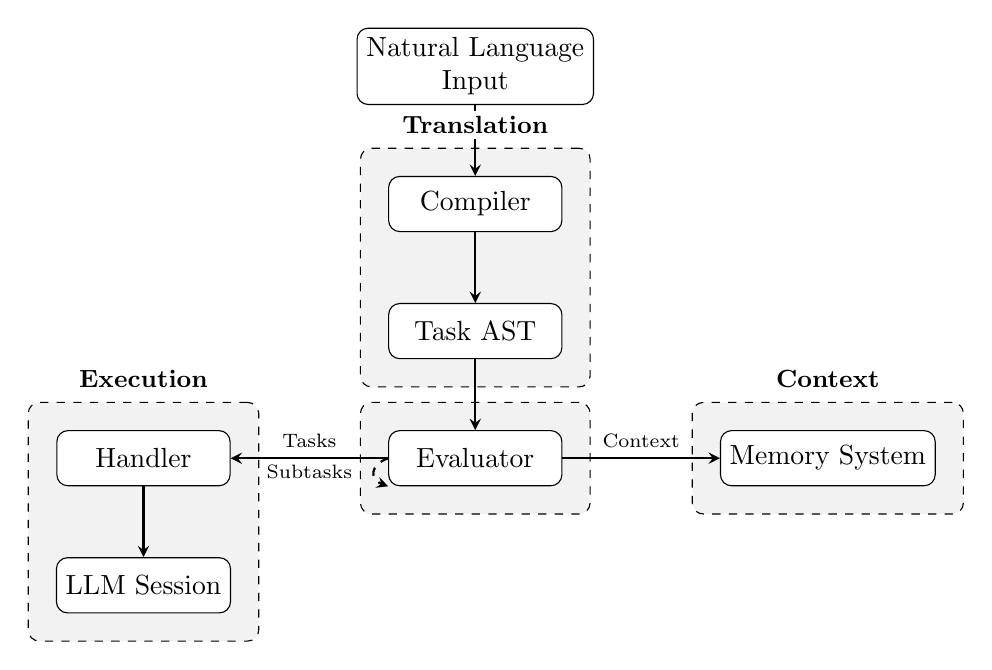
\begin{tikzpicture}[
    node distance=1.2cm,
    box/.style={draw, rounded corners, minimum width=2.2cm, minimum height=0.7cm, align=center, fill=white},
    arrow/.style={->, >=stealth, thick},
    group/.style={draw, dashed, rounded corners, inner sep=10pt, fill=gray!10},
    grouplabel/.style={font=\small\bfseries, fill=white, inner sep=2pt}
]
    % User input
    \node[box] (user) {Natural Language\\Input};
    
    % Main components - vertical flow with adjusted spacing
    \node[box, below=0.9cm of user] (compiler) {Compiler};
    \node[box, below=0.9cm of compiler] (ast) {Task AST};
    \node[box, below=0.9cm of ast] (evaluator) {Evaluator};
    
    % Systems - reduced horizontal spacing
    \node[box, right=2cm of evaluator] (memory) {Memory System};
    \node[box, left=2cm of evaluator] (handler) {Handler};
    
    % LLM - adjusted position
    \node[box, below=0.9cm of handler] (llm) {LLM Session};
    
    % Connections
    \draw[arrow] (user) -- (compiler);
    \draw[arrow] (compiler) -- (ast);
    \draw[arrow] (ast) -- (evaluator);
    \draw[arrow] (evaluator) -- (memory) node[midway, above, font=\scriptsize] {Context};
    \draw[arrow] (evaluator) -- (handler) node[midway, above, font=\scriptsize] {Tasks};
    \draw[arrow] (handler) -- (llm);
    
    % Curved arrow with safer positioning
    \draw[arrow, dashed] (evaluator.west) to[out=200, in=160, looseness=1.8] 
        node[midway, left, font=\scriptsize, xshift=-0.15cm] {Subtasks} (evaluator.south west);
    
    % Group boundaries with better spacing
    \begin{pgfonlayer}{background}
        \node[group, fit=(compiler)(ast)] (g1) {};
        \node[group, fit=(evaluator)] (g2) {};
        \node[group, fit=(memory)] (g3) {};
        \node[group, fit=(handler)(llm)] (g4) {};
    \end{pgfonlayer}
    
    % Add labels after the background layer to prevent them from being covered
    \node[grouplabel, above=0.1cm of g1] {Translation};
    \node[grouplabel, above=0.1cm of g3] {Context};
    \node[grouplabel, above=0.1cm of g4] {Execution};
\end{tikzpicture}

\vspace{0.2cm}
\textbf{Main components:}
\begin{itemize}\setlength{\itemsep}{0pt}
    \item \textbf{Compiler} – Translates natural language to structured tasks
    \item \textbf{Evaluator} – Manages task execution and resource usage
    \item \textbf{Memory system} – Maintains working context across operations
\end{itemize}

\end{frame}

% REVISED: Next Steps slide to be more open-ended
\begin{frame}
\frametitle{Potential Next Steps}

\begin{enumerate}
\item \textbf{Start small:} Prototype one-off tools for specific SLAC use cases
\item \textbf{Explore context management:} Data handling choices -- such as RAG vs. direct context management -- become important at large scales
\item \textbf{Consider domain-specific libraries:} Would building a library of SLAC-specific LLM primitives be valuable?
\end{enumerate}

\vspace{0.5cm}
\centering
\end{frame}

\end{document}
